\documentclass[border=0pt,10pt]{standalone}
\usepackage[T1]{fontenc}
\usepackage{lmodern}
\usepackage{pgfplots}
\pgfplotsset{compat=1.17}
\usepgfplotslibrary{groupplots}
\usepackage{xcolor}
\definecolor{oi-blue}{HTML}{0072B2}
\definecolor{oi-vermillion}{HTML}{D55E00}
\definecolor{oi-green}{HTML}{009E73}
\definecolor{oi-purple}{HTML}{CC79A7}
\definecolor{oi-black}{HTML}{000000}
% semantic_sha256: bd2a953e6fdeba82f892112e77e569b479863bd0d1672a21f119ca1f80c333bc
\begin{document}
\begin{minipage}{181.86mm}
\centering
{\bfseries\fontsize{10}{12}\selectfont PP-U-ARPLS | D2 | source\_fit}\\[2mm]
{\fontsize{8}{10}\selectfont planned=66, monitored=63, missing-history=3, status=partial\_history\_coverage}\\[3mm]
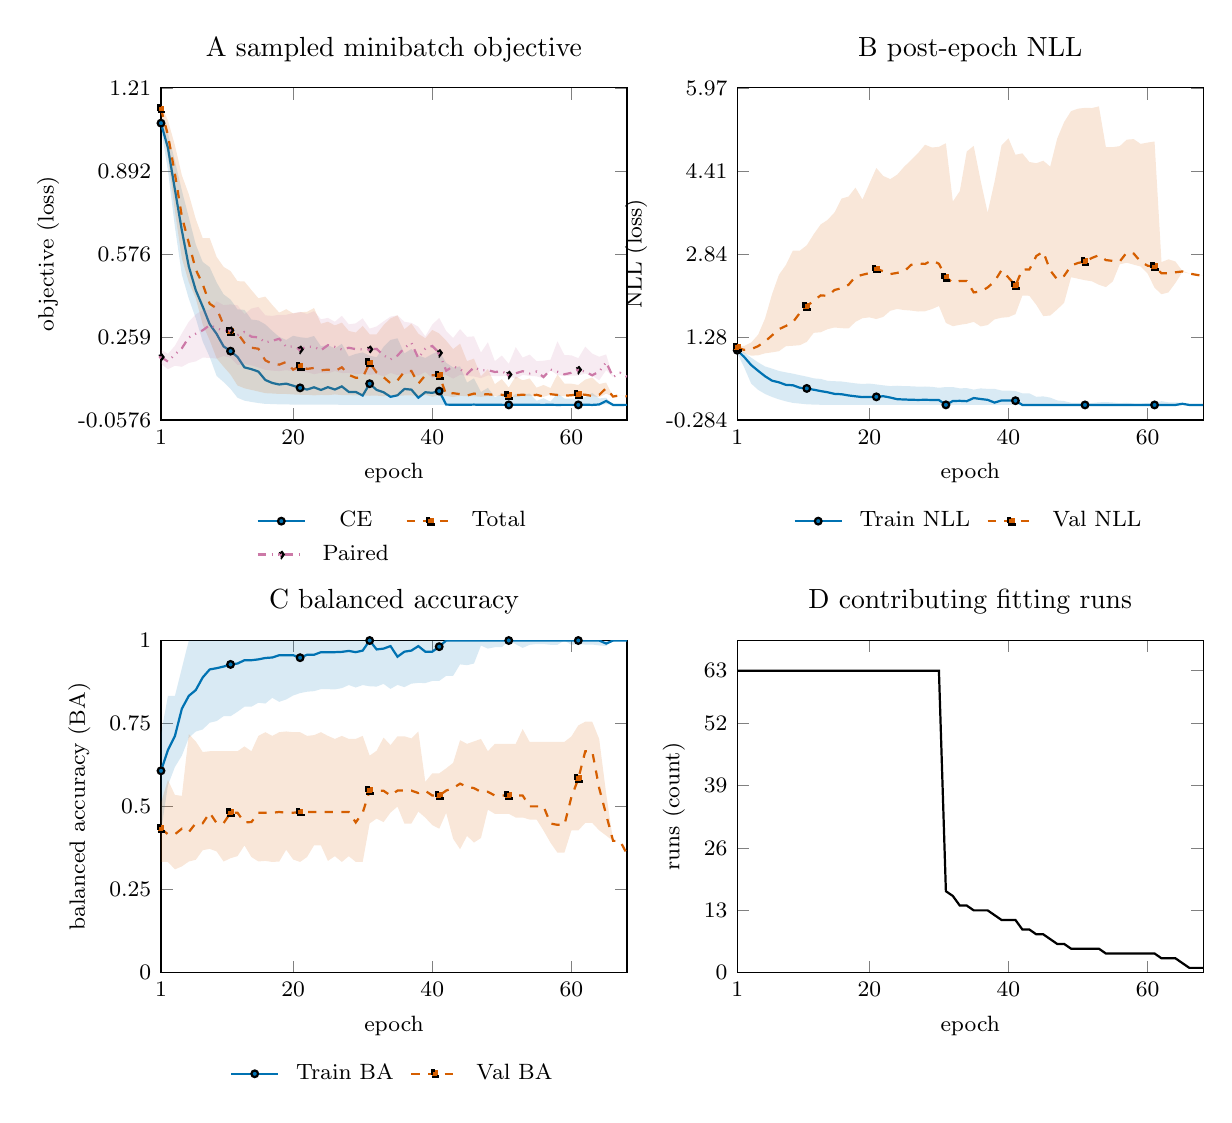
\begin{tikzpicture}
\begin{groupplot}[group style={group size=2 by 2, horizontal sep=14mm, vertical sep=28mm}]
\nextgroupplot[width=75mm, height=58mm, title={A sampled minibatch objective}, xlabel={epoch}, ylabel={objective (loss)}, xmin=1, xmax=68, xtick={1,20,40,60}, ymin=-0.057554432451725007, ymax=1.208643081486225, ytick={-0.057554432451725007,0.25899494603276252,0.57554432451725002,0.89209370300173751,1.208643081486225}, yticklabels={-0.0576,0.259,0.576,0.892,1.21}, tick label style={font=\fontsize{8}{9}\selectfont, text=black}, label style={font=\fontsize{8}{9}\selectfont, text=black}, title style={font=\fontsize{10}{11}\selectfont, text=black}, legend style={at={(0.5,-0.24)},anchor=north,draw=none,fill=none,font=\fontsize{8}{9}\selectfont,row sep=1pt,column sep=4pt,legend columns=2}]
\addplot[fill=oi-blue,opacity=0.15,draw=none,forget plot] coordinates {(1,1.0561847865581513) (2,0.89317666292190556) (3,0.67859060466289522) (4,0.49613250195980074) (5,0.40492118299007418) (6,0.3302676945924759) (7,0.24158049076795579) (8,0.18286470919847489) (9,0.11047817450016736) (10,0.087279613129794598) (11,0.06113896332681179) (12,0.027579788630828262) (13,0.016259650315623729) (14,0.011545587400905787) (15,0.0072016631020233035) (16,0.0040299443469848486) (17,0.003403825266286731) (18,0.0022276689123827964) (19,0.0019585356581956147) (20,0.0014314170344732701) (21,0.0013918561278842389) (22,0.0013536893253331074) (23,0.001082266071171034) (24,0.00086677130602765831) (25,0.0008853006089339033) (26,0.00096779873711057003) (27,0.00049005577457137404) (28,0.00052689329895656552) (29,0.00058395346495672136) (30,0.00027780428899859544) (31,0.00038170029438333586) (32,0.00029259271377668483) (33,0.00033172780731547394) (34,0.00031623275999663746) (35,0.00030415530018217395) (36,0.00030797364015597848) (37,0.00020047712096129546) (38,0.00022407798760468723) (39,0.00068782388188992627) (40,0.00030874503136146814) (41,0.00026326324950787239) (42,0.00019337330995767844) (43,0.00017393893103871959) (44,0.00016154482527781512) (45,0.00014252512273742467) (46,7.4651620707300026e-05) (47,7.5200154697085964e-05) (48,0.00017956302190214046) (49,0.00026096831861650572) (50,0.00023556586056656671) (51,0.00010210449672740652) (52,0.000102404226163344) (53,0.00023644874218007317) (54,0.00013450115575324164) (55,0.00017075325281439292) (56,7.4940750482710425e-05) (57,0.00011184972340743117) (58,6.9801053336959745e-05) (59,8.5610680253012111e-05) (60,5.5717189798087933e-05) (61,0.0001177975706923462) (62,0.00025856491374725015) (63,4.1151479581458259e-05) (64,0.00047010441704742334) (65,0.0031335959840362196) (66,8.0695571796240984e-05) (67,5.8122554037254304e-05) (68,0.0002951619035229669) (68,0.0002951619035229669) (67,5.8122554037254304e-05) (66,8.0695571796240984e-05) (65,0.027510044585869763) (64,0.024728564865665704) (63,0.045817113833891199) (62,0.029982577976443284) (61,0.022960949221442213) (60,0.024268725028741764) (59,0.024538242825838101) (58,0.043564142170043861) (57,0.012700136613057115) (56,0.02561466065526475) (55,0.015800554814268258) (54,0.043593246721411572) (53,0.039780203644477305) (52,0.042545035493094477) (51,0.019584992546879225) (50,0.042068271214520794) (49,0.0291062010335736) (48,0.065233232919126749) (47,0.049352259316947311) (46,0.10150933908298615) (45,0.085309973964467642) (44,0.14696100838482379) (43,0.14279710128903389) (42,0.16062024980783463) (41,0.2053222581744194) (40,0.19420438632369041) (39,0.17916016280651093) (38,0.18837216533720494) (37,0.2132212229073048) (36,0.19659763127565386) (35,0.25395306497812276) (34,0.24771154839545489) (33,0.22140229977667344) (32,0.18199034780263901) (31,0.18752209022641184) (30,0.20015378929674627) (29,0.19439041353762157) (28,0.18493725880980491) (27,0.23300050124526037) (26,0.21534060984849931) (25,0.2281172029674054) (24,0.22369463667273529) (23,0.26277252510190019) (22,0.25512244105339049) (21,0.25803015530109408) (20,0.26355505660176282) (19,0.24779014885425568) (18,0.25917879790067677) (17,0.281973572075367) (16,0.30705287083983424) (15,0.32213373929262168) (14,0.32556769549846648) (13,0.36247614771127701) (12,0.36438938975334167) (11,0.40157017558813096) (10,0.42149234563112259) (9,0.46691360473632815) (8,0.52522758841514594) (7,0.54495591819286349) (6,0.61151224076747901) (5,0.71500121355056767) (4,0.81763840317726144) (3,0.93077407181262972) (2,1.035999995470047) (1,1.0881977558135987)};
\addplot[color=oi-blue, mark=*, mark options={draw=black}, mark repeat=10, mark size=1.2pt, solid, line width=0.8pt] coordinates {(1,1.0741778016090393) (2,0.97974681854248047) (3,0.8213697075843811) (4,0.66501696407794952) (5,0.52778424322605133) (6,0.43728911131620407) (7,0.37465598434209824) (8,0.30800687521696091) (9,0.27070166915655136) (10,0.22301669046282768) (11,0.20500369742512703) (12,0.18290937226265669) (13,0.14318012446165085) (14,0.13649400696158409) (15,0.12720958236604929) (16,0.095146889798343182) (17,0.083807965740561485) (18,0.077914301306009293) (19,0.081219334853813052) (20,0.073366155847907066) (21,0.065134555101394653) (22,0.058701247908174992) (23,0.067239426076412201) (24,0.057083465158939362) (25,0.067777124233543873) (26,0.05878991587087512) (27,0.070625006686896086) (28,0.049708299338817596) (29,0.049486862029880285) (30,0.035986546892672777) (31,0.080941000720486045) (32,0.057344594155438244) (33,0.04845185112208128) (34,0.03095356680569239) (35,0.036781968548893929) (36,0.060993972234427929) (37,0.058333002496510744) (38,0.027570321843086276) (39,0.048414952121675014) (40,0.046121438033878803) (41,0.052840585354715586) (42,0.0013615661664516665) (43,0.00072545612056273967) (44,0.0004535622301773401) (45,0.00070546004462812562) (46,0.001327531470451504) (47,0.00037876117130508646) (48,0.00094861167872295482) (49,0.00045749161199637456) (50,0.00033384913876943756) (51,0.00015520257602474885) (52,0.00077756102473358624) (53,0.00049664818561723223) (54,0.00039276893949136138) (55,0.00040511234124096518) (56,0.00025075103417293576) (57,0.00053671124260290526) (58,7.5811508963852248e-05) (59,0.00029549220835178858) (60,0.00021235383428575005) (61,0.00029125345395186741) (62,0.00090607425499911187) (63,8.4845248693454778e-05) (64,0.0017474067572607055) (65,0.015321820284952992) (66,8.0695571796240984e-05) (67,5.8122554037254304e-05) (68,0.0002951619035229669)};
\addlegendentry{CE}
\addplot[fill=oi-vermillion,opacity=0.15,draw=none,forget plot] coordinates {(1,1.1131294310092925) (2,0.94411517977714543) (3,0.7387645483016968) (4,0.55863462090492244) (5,0.46826974898576734) (6,0.40669837146997451) (7,0.30610559284687044) (8,0.24653715565800666) (9,0.17797563858330251) (10,0.14596580900251865) (11,0.11573442295193673) (12,0.074191716127097601) (13,0.063541310280561453) (14,0.057288308627903461) (15,0.051281813345849511) (16,0.044845746178179977) (17,0.04364860486239195) (18,0.042022231407463549) (19,0.041933734621852639) (20,0.040018450841307639) (21,0.038773098960518837) (22,0.038655640184879304) (23,0.036453326605260371) (24,0.038128836639225484) (25,0.037303368747234347) (26,0.040123600140213968) (27,0.037496962212026121) (28,0.037333243526518345) (29,0.036448831390589478) (30,0.036216761544346811) (31,0.034974668826907876) (32,0.035632386570796371) (33,0.033101558173075321) (34,0.037280826736241578) (35,0.034332524053752422) (36,0.03623296683654189) (37,0.036410929728299381) (38,0.033662435971200465) (39,0.038622057531028986) (40,0.031130274757742882) (41,0.036182436626404524) (42,0.034593443199992177) (43,0.030172098614275455) (44,0.034721908299252389) (45,0.033273950126022099) (46,0.033386917505413297) (47,0.030960771953687072) (48,0.034019735641777515) (49,0.033288946934044363) (50,0.033339572511613368) (51,0.033436689898371695) (52,0.029897600505501033) (53,0.034801727067679165) (54,0.033580529876053332) (55,0.032871678937226534) (56,0.030741175357252359) (57,0.039823857508599757) (58,0.034269151417538522) (59,0.033178254636004566) (60,0.033604041999205948) (61,0.033890161011368033) (62,0.036233483999967578) (63,0.033464805036783216) (64,0.029603024758398534) (65,0.042947599198669195) (66,0.031995351426303387) (67,0.036804140545427799) (68,0.032556223217397928) (68,0.032556223217397928) (67,0.036804140545427799) (66,0.031995351426303387) (65,0.085300301667302847) (64,0.079565022327005866) (63,0.10451745502650739) (62,0.096688747778534895) (61,0.076372528728097688) (60,0.080991251859813942) (59,0.081614167662337436) (58,0.11633493499830366) (57,0.064419839903712278) (56,0.076107877586036932) (55,0.065840536821633586) (54,0.10108968615531923) (53,0.093801865912973889) (52,0.10858629401773215) (51,0.066565910540521148) (50,0.09860605616122485) (49,0.079130814783275133) (48,0.13694306183606386) (47,0.10931331058964133) (46,0.17670820839703089) (45,0.16694858893752099) (44,0.2336895652115345) (43,0.21280089169740679) (42,0.24519612491130829) (41,0.27238048613071442) (40,0.28609780967235565) (39,0.25430501252412796) (38,0.27166741974651815) (37,0.3103657498955727) (36,0.28836197778582573) (35,0.34152417033910754) (34,0.33001116849482065) (33,0.30441185608506216) (32,0.2692088820040226) (31,0.26943086385726928) (30,0.30120359510183337) (29,0.27600974887609486) (28,0.28210483342409137) (27,0.31370611041784296) (26,0.3032323077321053) (25,0.31731154918670657) (24,0.30950114727020267) (23,0.36920877695083626) (22,0.35511026009917263) (21,0.35340162813663489) (20,0.34875434637069708) (19,0.36502987667918207) (18,0.35190781205892563) (17,0.38122847676277172) (16,0.41297559738159184) (15,0.40681184679269788) (14,0.43805976510047917) (13,0.470514552295208) (12,0.4718710690736771) (11,0.51033768057823181) (10,0.52627522200346) (9,0.56416777223348624) (8,0.63606460690498368) (7,0.63578136861324308) (6,0.70852592289447791) (5,0.80272455215454108) (4,0.87554864585399628) (3,0.99004056453704836) (2,1.0843369156122209) (1,1.1427570641040803)};
\addplot[color=oi-vermillion, mark=square*, mark options={draw=black}, mark repeat=10, mark size=1.2pt, dashed, line width=0.8pt] coordinates {(1,1.1286857128143311) (2,1.0287820249795914) (3,0.88124427199363708) (4,0.71817420423030853) (5,0.61749887466430664) (6,0.51569433510303497) (7,0.45995547622442245) (8,0.38568611443042755) (9,0.36797428131103516) (10,0.30471306294202805) (11,0.2790297195315361) (12,0.27395894378423691) (13,0.236799456179142) (14,0.21820499375462532) (15,0.2143133357167244) (16,0.16982746869325638) (17,0.15714729763567448) (18,0.15358497947454453) (19,0.16391235310584307) (20,0.13445199280977249) (21,0.14812281727790833) (22,0.1373369675129652) (23,0.14103800524026155) (24,0.13201155420392752) (25,0.1346012270078063) (26,0.12873909063637257) (27,0.1434783935546875) (28,0.11471685580909252) (29,0.10363654047250748) (30,0.10479313507676125) (31,0.16037851385772228) (32,0.12327867466956377) (33,0.10594298364594579) (34,0.082593872211873531) (35,0.093184110708534718) (36,0.1276770792901516) (37,0.12979561276733875) (38,0.081063329242169857) (39,0.11279613152146339) (40,0.11351900920271873) (41,0.11231529153883457) (42,0.040107918903231621) (43,0.044794505462050438) (44,0.041159354615956545) (45,0.035934533458203077) (46,0.043383011594414711) (47,0.039809940848499537) (48,0.040719614131376147) (49,0.038185577373951674) (50,0.038564717397093773) (51,0.034886094741523266) (52,0.036955926567316055) (53,0.039125117938965559) (54,0.03620180394500494) (55,0.038610144983977079) (56,0.031947171548381448) (57,0.041035526432096958) (58,0.038058412494137883) (59,0.035326419631019235) (60,0.036978320684283972) (61,0.040446817874908447) (62,0.039000490680336952) (63,0.033960649743676186) (64,0.038381275720894337) (65,0.064123950432986021) (66,0.031995351426303387) (67,0.036804140545427799) (68,0.032556223217397928)};
\addlegendentry{Total}
\addplot[fill=oi-purple,opacity=0.15,draw=none,forget plot] coordinates {(1,0.15713580846786498) (2,0.13602466471493244) (3,0.1494760312139988) (4,0.14539577290415764) (5,0.1600942887365818) (6,0.16599115580320359) (7,0.18040307834744454) (8,0.1793821170926094) (9,0.17657520025968551) (10,0.18674071356654168) (11,0.17939754351973533) (12,0.15222743600606919) (13,0.15553619526326656) (14,0.15066469870507718) (15,0.14284641444683074) (16,0.13362125270068645) (17,0.13066469505429268) (18,0.1291060909628868) (19,0.13234920874238015) (20,0.12847602367401123) (21,0.12502092681825161) (22,0.12444853633642197) (23,0.11732971668243408) (24,0.12196715511381626) (25,0.1199159488081932) (26,0.12917269356548786) (27,0.12140243947505951) (28,0.1223052479326725) (29,0.11682528965175151) (30,0.11991346329450607) (31,0.11466631218791008) (32,0.11779930908232927) (33,0.10885487701743841) (34,0.12201822958886624) (35,0.11342789381742477) (36,0.11823249123990535) (37,0.12000790946185588) (38,0.11143778823316097) (39,0.12570240907371044) (40,0.10197840072214603) (41,0.11973057873547077) (42,0.11368922777473926) (43,0.10010862834751606) (44,0.11492261048406363) (45,0.11029012221843004) (46,0.10851427726447582) (47,0.10224758554250002) (48,0.11280057113617659) (49,0.10975827127695084) (50,0.110119054839015) (51,0.11110405921936035) (52,0.099317315593361849) (53,0.11445927880704403) (54,0.11077828630805016) (55,0.10900307986885309) (56,0.10144493151456117) (57,0.13237335458397864) (58,0.11397516578435898) (59,0.11030880827456713) (60,0.11182774566113948) (61,0.11183644682168961) (62,0.11991639398038387) (63,0.11141217686235905) (64,0.093916472792625424) (65,0.13271333780139685) (66,0.10638218186795712) (67,0.12248672172427177) (68,0.10753686726093292) (68,0.10753686726093292) (67,0.12248672172427177) (66,0.10638218186795712) (65,0.19263418074697256) (64,0.18385260701179504) (63,0.19566780067980291) (62,0.22235388718545437) (61,0.1783549163490534) (60,0.18907507993280889) (59,0.19025307465344668) (58,0.24257900267839433) (57,0.17239900529384614) (56,0.16864322684705257) (55,0.16679993197321893) (54,0.19181158784776928) (53,0.18060851246118548) (52,0.22013751417398453) (51,0.15660305544734002) (50,0.18845927789807321) (49,0.16687215268611907) (48,0.23903274722397327) (47,0.1998701598495245) (46,0.26138210818171503) (45,0.2595183402299881) (44,0.28909515775740147) (43,0.25535874143242837) (42,0.28191955611109737) (41,0.33153901621699333) (40,0.30631138011813164) (39,0.2617134191095829) (38,0.29822242036461832) (37,0.31282871365547182) (36,0.31694129779934882) (35,0.34149917587637901) (34,0.33664523288607606) (33,0.31865500472486025) (32,0.29926100187003613) (31,0.29086099788546566) (30,0.33013663887977601) (29,0.31098886504769324) (28,0.30721271187067034) (27,0.33992547839879989) (26,0.31725762411952024) (25,0.33177512958645822) (24,0.32645801752805709) (23,0.3572811767458916) (22,0.34650577902793889) (21,0.35488853827118871) (20,0.34979753196239471) (19,0.34374276697635653) (18,0.34370283335447316) (17,0.33938247263431554) (16,0.34146055579185486) (15,0.37355083972215658) (14,0.36740488111972808) (13,0.34612319022417071) (12,0.37983516007661822) (11,0.38347872346639633) (10,0.38062611743807795) (9,0.39541530311107642) (8,0.36240670233964922) (7,0.36141161248087883) (6,0.34521984755992891) (5,0.31728345900774002) (4,0.2728398457169533) (3,0.22549935430288318) (2,0.19476149827241898) (1,0.210348991304636)};
\addplot[color=oi-purple, mark=diamond*, mark options={draw=black}, mark repeat=10, mark size=1.2pt, dash dot dot, line width=0.8pt] coordinates {(1,0.18267116323113441) (2,0.16526507958769798) (3,0.19269822165369987) (4,0.21615755185484886) (5,0.25727253779768944) (6,0.27164663746953011) (7,0.28468659520149231) (8,0.3038967028260231) (9,0.29288500919938087) (10,0.28217223659157753) (11,0.28463838621973991) (12,0.26631298661231995) (13,0.27800008654594421) (14,0.2602166049182415) (15,0.2574256993830204) (16,0.2382538877427578) (17,0.24445150792598724) (18,0.25223560258746147) (19,0.22202092036604881) (20,0.22352727502584457) (21,0.21175210177898407) (22,0.22243471816182137) (23,0.22188713774085045) (24,0.20831670612096786) (25,0.2279527485370636) (26,0.22133483365178108) (27,0.21129077300429344) (28,0.21796417981386185) (29,0.21281185373663902) (30,0.21188865229487419) (31,0.21207447350025177) (32,0.21381375007331371) (33,0.18885587714612484) (34,0.17396634072065353) (35,0.18800713121891022) (36,0.21726732328534126) (37,0.23669873923063278) (38,0.17831001989543438) (39,0.21460393443703651) (40,0.2246585488319397) (41,0.19824900850653648) (42,0.13055791333317757) (43,0.14689682424068451) (44,0.13637525774538517) (45,0.11752246972173452) (46,0.14376622997224331) (47,0.13214157801121473) (48,0.13257000409066677) (49,0.1257602795958519) (50,0.12781560607254505) (51,0.11579768545925617) (52,0.12059454619884491) (53,0.12876155786216259) (54,0.12005303520709276) (55,0.127350103110075) (56,0.10620890744030476) (57,0.13499604351818562) (58,0.12662485428154469) (59,0.11676975432783365) (60,0.12255321815609932) (61,0.13437908794730902) (62,0.12698139064013958) (63,0.11291934736073017) (64,0.12743498384952545) (65,0.1626737592741847) (66,0.10638218186795712) (67,0.12248672172427177) (68,0.10753686726093292)};
\addlegendentry{Paired}
\nextgroupplot[width=75mm, height=58mm, title={B post-epoch NLL}, xlabel={epoch}, ylabel={NLL (loss)}, xmin=1, xmax=68, xtick={1,20,40,60}, ymin=-0.28430119507859269, ymax=5.9703250966504458, ytick={-0.28430119507859269,1.2793553778536668,2.8430119507859266,4.406668523718186,5.9703250966504458}, yticklabels={-0.284,1.28,2.84,4.41,5.97}, tick label style={font=\fontsize{8}{9}\selectfont, text=black}, label style={font=\fontsize{8}{9}\selectfont, text=black}, title style={font=\fontsize{10}{11}\selectfont, text=black}, legend style={at={(0.5,-0.24)},anchor=north,draw=none,fill=none,font=\fontsize{8}{9}\selectfont,row sep=1pt,column sep=4pt,legend columns=2}]
\addplot[fill=oi-blue,opacity=0.15,draw=none,forget plot] coordinates {(1,0.97701385983165245) (2,0.70707829825786384) (3,0.4027124646216938) (4,0.28432196284982481) (5,0.20658298421548921) (6,0.15026221045084137) (7,0.10489032553271969) (8,0.067594224341057579) (9,0.038148455440040439) (10,0.025143324720482627) (11,0.011910883423523713) (12,0.0063936280323542418) (13,0.0028031533072212581) (14,0.0014718967473290087) (15,0.0012798350187388295) (16,0.00079450768538700796) (17,0.0005302696666547815) (18,0.00035386248326189603) (19,0.000255356310839252) (20,0.00020558306678964113) (21,0.00016014895240558551) (22,0.00015396438206536004) (23,0.0001298182156474158) (24,0.00012424096868976779) (25,9.8564659934121429e-05) (26,8.0822009973145715e-05) (27,6.8850286817151701e-05) (28,5.9516516467260063e-05) (29,4.8077508262255397e-05) (30,4.1430117537002363e-05) (31,3.3344845937323017e-05) (32,3.3582152431155661e-05) (33,3.2862850031597449e-05) (34,3.0772829486588794e-05) (35,2.6731249664091039e-05) (36,2.7040098059439758e-05) (37,2.563126224198584e-05) (38,2.4750750829252127e-05) (39,2.1520467635521368e-05) (40,2.3886767244572384e-05) (41,2.5255233201548639e-05) (42,2.3280008854438203e-05) (43,1.9540920631984536e-05) (44,1.6744577828349155e-05) (45,1.4661975742597389e-05) (46,1.7945372188657442e-05) (47,1.7422652058040555e-05) (48,1.4775747834760385e-05) (49,1.3004109064873792e-05) (50,1.188414405247215e-05) (51,1.1090078609905449e-05) (52,1.0264282846725312e-05) (53,9.5007597494382364e-06) (54,8.6574174280117683e-06) (55,8.2761936256520719e-06) (56,8.1240887609557832e-06) (57,7.980307437293825e-06) (58,7.8184392307767756e-06) (59,7.1671380924305088e-06) (60,6.619150214658021e-06) (61,6.1635427994371074e-06) (62,5.971506602907104e-06) (63,5.6760501084843347e-06) (64,4.7378288963308286e-06) (65,0.0042901905077256481) (66,4.8927851712144828e-06) (67,4.8880565522474554e-06) (68,5.3314894101362639e-06) (68,5.3314894101362639e-06) (67,4.8880565522474554e-06) (66,4.8927851712144828e-06) (65,0.03857208231172065) (64,0.049043923379181467) (63,0.049117284623254459) (62,0.071679605232338003) (61,0.028971775588126157) (60,0.037165283490264586) (59,0.024101618870569181) (58,0.027103928942594814) (57,0.041370516735427923) (56,0.033036053717064542) (55,0.045834324734852896) (54,0.054640641074945609) (53,0.049201494251586778) (52,0.036574066718002202) (51,0.034761526316520824) (50,0.037209739719486622) (49,0.039699406890851469) (48,0.073632418908850472) (47,0.085242295793005893) (46,0.13797191231873346) (45,0.16125908112349602) (44,0.15287627142807425) (43,0.21803743994518202) (42,0.21767549190473082) (41,0.26171035151968869) (40,0.27094072476654107) (39,0.27140432216886218) (38,0.30242269650811648) (37,0.30241777247139434) (36,0.3114902039387013) (35,0.28858726731507672) (34,0.31667619257872959) (33,0.31224479925296283) (32,0.33657864216123495) (31,0.33692884717244187) (30,0.32328348405907076) (29,0.34031450624473131) (28,0.34729438124697826) (27,0.34425655112541287) (26,0.35169894221657994) (25,0.35374144574248512) (24,0.36160890626682141) (23,0.35483079983735077) (22,0.36912695826252823) (21,0.38633373299366935) (20,0.40198216813937226) (19,0.39536672473293422) (18,0.40652353401743624) (17,0.42373582721755287) (16,0.44147472072075677) (15,0.44678364903105539) (14,0.45368819556226225) (13,0.49019644835304393) (12,0.50034609664425456) (11,0.53324446870070574) (10,0.56013332461734644) (9,0.58949569643191491) (8,0.61307036465973141) (7,0.64036263907675162) (6,0.68421217587999783) (5,0.72469520875394977) (4,0.80179595333901876) (3,0.89095601659534973) (2,0.98726394399330153) (1,1.0663368812580283)};
\addplot[color=oi-blue, mark=*, mark options={draw=black}, mark repeat=10, mark size=1.2pt, solid, line width=0.8pt] coordinates {(1,1.0297755377063349) (2,0.90301575257478628) (3,0.75201918854199745) (4,0.64269527074808075) (5,0.54039683577784869) (6,0.4570192131600192) (7,0.42581514974134294) (8,0.37795172217543993) (9,0.37075701102171493) (10,0.32339645988859328) (11,0.31068193436916591) (12,0.28649314649809809) (13,0.26094065297683627) (14,0.23838540565090161) (15,0.20811893781864729) (16,0.20165604093114617) (17,0.17881947279421073) (18,0.1625904898547606) (19,0.14725031010174044) (20,0.14987519841890459) (21,0.15263188580297471) (22,0.16445037657063039) (23,0.1391476908402752) (24,0.10808353758758735) (25,0.10237593227800516) (26,0.097035228340711627) (27,0.094503149185529448) (28,0.096605624963209916) (29,0.094068999206840642) (30,0.091715563153631788) (31,0.0015998408705058939) (32,0.074218460851021323) (33,0.077383766984390381) (34,0.070778726973975331) (35,0.12984932318793732) (36,0.11171138406879445) (37,0.095880316263385681) (38,0.04402375126447703) (39,0.08472562040195758) (40,0.084766975938191796) (41,0.079970273347735987) (42,7.476303124930775e-05) (43,0.00011821798099364307) (44,8.2270976253385515e-05) (45,6.137218025801657e-05) (46,5.7391494595312277e-05) (47,2.8692676819399526e-05) (48,2.5179755955424226e-05) (49,2.0720134655386439e-05) (50,2.0997653476835038e-05) (51,2.0089065304031416e-05) (52,2.0246657749213642e-05) (53,1.7000683100244369e-05) (54,1.2242295104298642e-05) (55,1.1486963850077881e-05) (56,1.0621958639423293e-05) (57,1.0095812271756205e-05) (58,9.6623374463827195e-06) (59,9.2048999835116284e-06) (60,8.5891689205432892e-06) (61,7.8867686991576571e-06) (62,7.4627741702157834e-06) (63,6.8641423745193166e-06) (64,5.1165405107960414e-06) (65,0.021431136409723148) (66,4.8927851712144828e-06) (67,4.8880565522474554e-06) (68,5.3314894101362639e-06)};
\addlegendentry{Train NLL}
\addplot[fill=oi-vermillion,opacity=0.15,draw=none,forget plot] coordinates {(1,1.0378117752639995) (2,0.97197290271252534) (3,0.92804546054569148) (4,0.93431371526741158) (5,0.97220797003523418) (6,0.99052811590576861) (7,1.0116488642922392) (8,1.1065270165964736) (9,1.1144592994119509) (10,1.1251217958822179) (11,1.1873886694397919) (12,1.358093645709219) (13,1.3684320967184924) (14,1.4273995159156312) (15,1.4585058649304388) (16,1.44515496843971) (17,1.4400482593796551) (18,1.5639977391024784) (19,1.6330736436115552) (20,1.6486556642752173) (21,1.6180345311062245) (22,1.6579449471898313) (23,1.7728431132851281) (24,1.8071032117894454) (25,1.7866916190881246) (26,1.7770039661638715) (27,1.7592654508533077) (28,1.763594181491662) (29,1.8056086189280272) (30,1.8619832693751204) (31,1.5453735542884262) (32,1.4820313409530792) (33,1.5085064673844939) (34,1.5282294586092864) (35,1.5641164124587097) (36,1.4789209517637181) (37,1.5036295810432636) (38,1.6117230355212571) (39,1.6420315622387402) (40,1.6535749519128555) (41,1.7089548922957634) (42,2.0607175994740956) (43,2.0553774734960841) (44,1.8842931131128446) (45,1.6727988734467147) (46,1.684226797942606) (47,1.7969251667662189) (48,1.9245918991410309) (49,2.4051977550773138) (50,2.3770113539532383) (51,2.348284611554956) (52,2.3283250354469276) (53,2.2630263839187212) (54,2.2189391444622455) (55,2.325712016059414) (56,2.6479961400081469) (57,2.6778163663963594) (58,2.6417211700352392) (59,2.6059483238934735) (60,2.4745321829588418) (61,2.2068763238683498) (62,2.084395631837209) (63,2.1192470545729964) (64,2.2960871681981758) (65,2.5038954841601258) (66,2.474843601473153) (67,2.4503874493918838) (68,2.4316842163801553) (68,2.4316842163801553) (67,2.4503874493918838) (66,2.474843601473153) (65,2.5233917646521489) (64,2.7014802807543941) (63,2.741848879537395) (62,2.6901414452516463) (61,4.9604934601689159) (60,4.9404577074839668) (59,4.9156821786109779) (58,5.0058719624882242) (57,4.9955904022509037) (56,4.8735155221664055) (55,4.8546560336043987) (54,4.8554986709169903) (53,5.6215398046942679) (52,5.5909275743398252) (51,5.5939369707174187) (50,5.5792151920597473) (49,5.5330908848806093) (48,5.3278503910797772) (47,5.0146648121227528) (46,4.4881734345851134) (45,4.5985100059132771) (44,4.5518290359631903) (43,4.5752945456164769) (42,4.7372266472991305) (41,4.7117289158876057) (40,5.0194358878146526) (39,4.8890972321217534) (38,4.2070309937798829) (37,3.6216703463145463) (36,4.2212764566641034) (35,4.8774044641735195) (34,4.772879422963797) (33,4.0252521204330316) (32,3.8312978408638987) (31,4.9272596110709763) (30,4.860892824483388) (29,4.8467975031143808) (28,4.9001274250211457) (27,4.7419098267358324) (26,4.6103388802117857) (25,4.485673340772105) (24,4.3374883382496758) (23,4.25209022947835) (22,4.3117589961938725) (21,4.4609365847807689) (20,4.16625667785173) (19,3.8681731837601214) (18,4.0924324079759549) (17,3.9236898635853121) (16,3.8859928920281677) (15,3.62680921505503) (14,3.4856688743503494) (13,3.3987814626834996) (12,3.2153677993667551) (11,3.0068633642287828) (10,2.9056884192105001) (9,2.9078083358647482) (8,2.6361190532984207) (7,2.4520935658203005) (6,2.0836838349207256) (5,1.6274371412212829) (4,1.3213706522700899) (3,1.1749326736580317) (2,1.1116560283150554) (1,1.109138795297564)};
\addplot[color=oi-vermillion, mark=square*, mark options={draw=black}, mark repeat=10, mark size=1.2pt, dashed, line width=0.8pt] coordinates {(1,1.0803598567673693) (2,1.036117869398534) (3,1.0497899057739459) (4,1.1069804026854866) (5,1.1943560407350735) (6,1.3093142730497698) (7,1.4261157989340483) (8,1.4875158644534223) (9,1.5584972912306112) (10,1.7330272514952543) (11,1.8574800130786118) (12,1.9643335395572554) (13,2.0632212087024442) (14,2.0540007813753087) (15,2.1652675917665065) (16,2.1984771174722857) (17,2.262402470957289) (18,2.4152320252988297) (19,2.4507439178723032) (20,2.4817814100832405) (21,2.5609360837150521) (22,2.5188055770676647) (23,2.4639847115791453) (24,2.4867546381944168) (25,2.5124611939197918) (26,2.6380761730872271) (27,2.6616637050898944) (28,2.6556877103743277) (29,2.7233552980636526) (30,2.657053715869417) (31,2.4052710646571103) (32,2.3020892039695795) (33,2.3352298190060718) (34,2.3319310053386095) (35,2.1197742966190902) (36,2.1345339924431661) (37,2.212031503467133) (38,2.3270237352643077) (39,2.5380862869950525) (40,2.3979727424894253) (41,2.2466957087831849) (42,2.5539169011126068) (43,2.5499872505012711) (44,2.8050485145615109) (45,2.8850176531362828) (46,2.5327610405307297) (47,2.3634206359367709) (48,2.4298878569260309) (49,2.624710582311109) (50,2.6734529763688348) (51,2.7023305263793693) (52,2.7682574617560598) (53,2.8194496861954383) (54,2.7275968408684506) (55,2.7126651215447763) (56,2.7018777908279419) (57,2.8699688926520484) (58,2.8512570153245402) (59,2.6980292838670805) (60,2.6217863212657662) (61,2.6010973659915733) (62,2.4794244449686382) (63,2.4798187521754143) (64,2.4977445844111812) (65,2.5136436244061375) (66,2.474843601473153) (67,2.4503874493918838) (68,2.4316842163801553)};
\addlegendentry{Val NLL}
\nextgroupplot[width=75mm, height=58mm, title={C balanced accuracy}, xlabel={epoch}, ylabel={balanced accuracy (BA)}, xmin=1, xmax=68, xtick={1,20,40,60}, ymin=0, ymax=1, ytick={0,0.25,0.5,0.75,1}, yticklabels={0,0.25,0.5,0.75,1}, tick label style={font=\fontsize{8}{9}\selectfont, text=black}, label style={font=\fontsize{8}{9}\selectfont, text=black}, title style={font=\fontsize{10}{11}\selectfont, text=black}, legend style={at={(0.5,-0.24)},anchor=north,draw=none,fill=none,font=\fontsize{8}{9}\selectfont,row sep=1pt,column sep=4pt,legend columns=2}]
\addplot[fill=oi-blue,opacity=0.15,draw=none,forget plot] coordinates {(1,0.42532375032375036) (2,0.56429349727595335) (3,0.61918555778204898) (4,0.65349650349650357) (5,0.7072698767616209) (6,0.72587412587412581) (7,0.73230413377472203) (8,0.75256410256410267) (9,0.75749841556293174) (10,0.77213972805370656) (11,0.77206750364645105) (12,0.78555102305102309) (13,0.80074035880487493) (14,0.80074035880487493) (15,0.81271532236444521) (16,0.81019773761001834) (17,0.8274516333339863) (18,0.81534690131181364) (19,0.82253574885153824) (20,0.83438552188552195) (21,0.84171199171199174) (22,0.84591293047433402) (23,0.84750388500388496) (24,0.85365190365190358) (25,0.85343434343434332) (26,0.85290404040404033) (27,0.85664335664335667) (28,0.86594379467186489) (29,0.85850344424905833) (30,0.86586354821648948) (31,0.86222361946046155) (32,0.86129357565761078) (33,0.86944736955701873) (34,0.85426967038809143) (35,0.86636614684860302) (36,0.85957602339181283) (37,0.87010233918128643) (38,0.87244433198380567) (39,0.87179487179487181) (40,0.87828947368421051) (41,0.87828947368421051) (42,0.89360661268556008) (43,0.89360661268556008) (44,0.92815332815332807) (45,0.92579642579642585) (46,0.93069153069153066) (47,0.98484848484848486) (48,0.97558922558922556) (49,0.97979797979797978) (50,0.97979797979797978) (51,1) (52,0.98888888888888893) (53,0.97777777777777775) (54,0.98703703703703705) (55,0.98939393939393938) (56,0.98939393939393938) (57,0.98703703703703705) (58,0.98703703703703705) (59,1) (60,0.98703703703703705) (61,0.98939393939393938) (62,0.98787878787878791) (63,0.98787878787878791) (64,0.98518518518518516) (65,0.98333333333333339) (66,1) (67,1) (68,1) (68,1) (67,1) (66,1) (65,0.99814814814814812) (64,1) (63,1) (62,1) (61,1) (60,1) (59,1) (58,1) (57,1) (56,1) (55,1) (54,1) (53,1) (52,1) (51,1) (50,1) (49,1) (48,1) (47,1) (46,1) (45,1) (44,1) (43,1) (42,1) (41,1) (40,1) (39,1) (38,1) (37,1) (36,1) (35,1) (34,1) (33,1) (32,1) (31,1) (30,1) (29,1) (28,1) (27,1) (26,1) (25,1) (24,1) (23,1) (22,1) (21,1) (20,1) (19,1) (18,1) (17,1) (16,1) (15,1) (14,1) (13,1) (12,1) (11,1) (10,1) (9,1) (8,1) (7,1) (6,1) (5,1) (4,0.91666666666666663) (3,0.83333333333333337) (2,0.83333333333333337) (1,0.71893939393939388)};
\addplot[color=oi-blue, mark=*, mark options={draw=black}, mark repeat=10, mark size=1.2pt, solid, line width=0.8pt] coordinates {(1,0.6077441077441077) (2,0.67046783625730999) (3,0.71228070175438596) (4,0.79469696969696979) (5,0.83333333333333337) (6,0.85084033613445387) (7,0.88888888888888884) (8,0.91287878787878796) (9,0.91666666666666663) (10,0.92156862745098034) (11,0.92803030303030309) (12,0.93070175438596492) (13,0.94065656565656575) (14,0.94065656565656575) (15,0.94318181818181823) (16,0.94736842105263153) (17,0.94887955182072836) (18,0.95580808080808077) (19,0.95580808080808077) (20,0.95580808080808077) (21,0.94824561403508767) (22,0.95707070707070707) (23,0.95707070707070707) (24,0.96491228070175439) (25,0.96491228070175439) (26,0.96491228070175439) (27,0.96578947368421053) (28,0.96866096866096862) (29,0.96491228070175439) (30,0.96969696969696972) (31,1) (32,0.9731481481481481) (33,0.97558922558922556) (34,0.98316498316498313) (35,0.95117845117845123) (36,0.96632996632996626) (37,0.96969696969696972) (38,0.98316498316498313) (39,0.96632996632996626) (40,0.96632996632996626) (41,0.98148148148148151) (42,1) (43,1) (44,1) (45,1) (46,1) (47,1) (48,1) (49,1) (50,1) (51,1) (52,1) (53,1) (54,1) (55,1) (56,1) (57,1) (58,1) (59,1) (60,1) (61,1) (62,1) (63,1) (64,1) (65,0.9907407407407407) (66,1) (67,1) (68,1)};
\addlegendentry{Train BA}
\addplot[fill=oi-vermillion,opacity=0.15,draw=none,forget plot] coordinates {(1,0.33333333333333331) (2,0.33333333333333331) (3,0.31095238095238098) (4,0.32000000000000001) (5,0.33463203463203461) (6,0.33982683982683981) (7,0.36868686868686862) (8,0.37277056277056275) (9,0.36493506493506489) (10,0.33463203463203461) (11,0.34458874458874456) (12,0.35079365079365082) (13,0.38296296296296295) (14,0.34815776815776817) (15,0.33481481481481479) (16,0.33650793650793648) (17,0.33333333333333331) (18,0.33463203463203461) (19,0.37012987012987014) (20,0.34069264069264071) (21,0.33333333333333331) (22,0.34815776815776817) (23,0.38296296296296295) (24,0.38296296296296295) (25,0.33650793650793648) (26,0.35079365079365082) (27,0.33333333333333331) (28,0.35079365079365082) (29,0.33333333333333331) (30,0.33333333333333331) (31,0.44920634920634922) (32,0.46388888888888891) (33,0.45333333333333331) (34,0.48185185185185181) (35,0.5) (36,0.44888888888888884) (37,0.44888888888888884) (38,0.48499999999999999) (39,0.46666666666666662) (40,0.44444444444444442) (41,0.43333333333333335) (42,0.48095238095238096) (43,0.40328042328042324) (44,0.37158730158730158) (45,0.41179894179894178) (46,0.39174603174603173) (47,0.40537240537240538) (48,0.49068986568986572) (49,0.47826617826617823) (50,0.47826617826617823) (51,0.47826617826617823) (52,0.46715506715506716) (53,0.46715506715506716) (54,0.46111111111111108) (55,0.46111111111111108) (56,0.42777777777777776) (57,0.39126984126984121) (58,0.3611111111111111) (59,0.3611111111111111) (60,0.42814407814407812) (61,0.42814407814407812) (62,0.45079365079365075) (63,0.45079365079365075) (64,0.42857142857142855) (65,0.41269841269841268) (66,0.3968253968253968) (67,0.3968253968253968) (68,0.35714285714285715) (68,0.35714285714285715) (67,0.3968253968253968) (66,0.3968253968253968) (65,0.53968253968253965) (64,0.70370370370370372) (63,0.75555555555555554) (62,0.75555555555555554) (61,0.74444444444444446) (60,0.71111111111111114) (59,0.6948107448107449) (58,0.6948107448107449) (57,0.6948107448107449) (56,0.6948107448107449) (55,0.6948107448107449) (54,0.6948107448107449) (53,0.73333333333333339) (52,0.68888888888888888) (51,0.68888888888888888) (50,0.68888888888888888) (49,0.68888888888888888) (48,0.66666666666666663) (47,0.70370370370370372) (46,0.6962962962962963) (45,0.68888888888888888) (44,0.69999999999999996) (43,0.63174603174603172) (42,0.61514041514041518) (41,0.6001221001221001) (40,0.6001221001221001) (39,0.57448107448107455) (38,0.72619047619047628) (37,0.70531986531986546) (36,0.71164021164021185) (35,0.71164021164021185) (34,0.68518518518518545) (33,0.7076094276094278) (32,0.66798941798941802) (31,0.65343915343915349) (30,0.71286195286195297) (29,0.70370370370370372) (28,0.70370370370370372) (27,0.71286195286195297) (26,0.70370370370370372) (25,0.71286195286195297) (24,0.72398268398268406) (23,0.7151515151515152) (22,0.71286195286195297) (21,0.72398268398268406) (20,0.72398268398268406) (19,0.72619047619047628) (18,0.72398268398268406) (17,0.71286195286195297) (16,0.72398268398268406) (15,0.71286195286195297) (14,0.66666666666666663) (13,0.68121212121212138) (12,0.66666666666666663) (11,0.66666666666666663) (10,0.66666666666666663) (9,0.66666666666666663) (8,0.66666666666666663) (7,0.6642424242424243) (6,0.69629629629629641) (5,0.71792207792207818) (4,0.53222222222222226) (3,0.53523809523809518) (2,0.58000000000000007) (1,0.51190476190476186)};
\addplot[color=oi-vermillion, mark=square*, mark options={draw=black}, mark repeat=10, mark size=1.2pt, dashed, line width=0.8pt] coordinates {(1,0.43333333333333335) (2,0.41666666666666669) (3,0.41666666666666669) (4,0.43333333333333335) (5,0.42316017316017313) (6,0.44999999999999996) (7,0.44999999999999996) (8,0.48148148148148145) (9,0.44999999999999996) (10,0.44999999999999996) (11,0.48148148148148145) (12,0.48148148148148145) (13,0.45238095238095238) (14,0.45346320346320351) (15,0.48148148148148145) (16,0.48148148148148145) (17,0.48148148148148145) (18,0.48376623376623379) (19,0.48148148148148145) (20,0.48148148148148145) (21,0.48376623376623379) (22,0.48376623376623379) (23,0.48376623376623379) (24,0.48376623376623379) (25,0.48376623376623379) (26,0.48376623376623379) (27,0.48376623376623379) (28,0.48376623376623379) (29,0.45238095238095238) (30,0.4814814814814814) (31,0.54814814814814816) (32,0.54814814814814816) (33,0.54761904761904756) (34,0.53333333333333333) (35,0.54814814814814816) (36,0.54814814814814816) (37,0.54814814814814816) (38,0.54074074074074074) (39,0.54761904761904756) (40,0.53333333333333333) (41,0.53333333333333333) (42,0.54814814814814816) (43,0.55555555555555547) (44,0.56905871905871908) (45,0.55959595959595954) (46,0.55555555555555547) (47,0.5444444444444444) (48,0.5444444444444444) (49,0.53333333333333333) (50,0.53333333333333333) (51,0.53333333333333333) (52,0.53333333333333333) (53,0.53333333333333333) (54,0.50061050061050061) (55,0.50061050061050061) (56,0.50061050061050061) (57,0.44902319902319898) (58,0.44505494505494503) (59,0.44505494505494503) (60,0.52838827838827829) (61,0.58394383394383387) (62,0.66666666666666663) (63,0.66666666666666663) (64,0.55555555555555547) (65,0.47619047619047616) (66,0.3968253968253968) (67,0.3968253968253968) (68,0.35714285714285715)};
\addlegendentry{Val BA}
\nextgroupplot[width=75mm, height=58mm, title={D contributing fitting runs}, xlabel={epoch}, ylabel={runs (count)}, xmin=1, xmax=68, xtick={1,20,40,60}, ymin=0, ymax=69.300000000000011, ytick={0,13,26,39,52,63}, yticklabels={0,13,26,39,52,63}, tick label style={font=\fontsize{8}{9}\selectfont, text=black}, label style={font=\fontsize{8}{9}\selectfont, text=black}, title style={font=\fontsize{10}{11}\selectfont, text=black}]
\addplot[color=oi-black, solid, line width=0.8pt] coordinates {(1,63) (2,63) (3,63) (4,63) (5,63) (6,63) (7,63) (8,63) (9,63) (10,63) (11,63) (12,63) (13,63) (14,63) (15,63) (16,63) (17,63) (18,63) (19,63) (20,63) (21,63) (22,63) (23,63) (24,63) (25,63) (26,63) (27,63) (28,63) (29,63) (30,63) (31,17) (32,16) (33,14) (34,14) (35,13) (36,13) (37,13) (38,12) (39,11) (40,11) (41,11) (42,9) (43,9) (44,8) (45,8) (46,7) (47,6) (48,6) (49,5) (50,5) (51,5) (52,5) (53,5) (54,4) (55,4) (56,4) (57,4) (58,4) (59,4) (60,4) (61,4) (62,3) (63,3) (64,3) (65,2) (66,1) (67,1) (68,1)};
\end{groupplot}
\end{tikzpicture}
\par\vspace{6mm}
\begin{minipage}{175mm}
{\fontsize{8}{10}\selectfont RQ-S01 / Scope E: descriptive training diagnostics. 400-1800 cm-1 inputs: SG uses impulse replacement and Savitzky-Golay smoothing; arPLS uses impulse replacement and baseline correction; both finish with [0,1] min-max scaling. CE = chemical cross-entropy; SupCon = supervised contrastive; Paired = paired consistency; NLL = negative log-likelihood; BA = balanced accuracy. Authenticated complete monitor histories aggregated across unique fitting jobs into descriptive policy/recipe/stage curves. Curves summarize per-epoch minibatch-weighted training chemical cross-entropy and the composite total optimization objective; these sampled minibatch objectives differ from post-epoch evaluation negative log-likelihood. Auxiliary supcon/paired loss components are recipe-specific and are not directly comparable to the total objective across recipes. Validation metrics are recorded for source\_fit runs only and never substitute for a held-out test set; calibration\_model\_fit and final\_refit rows carry training-only diagnostics. Source\_fit optimization uses a 30-epoch minimum stopping threshold and a 200-epoch maximum; refit stages reuse the caller-selected duration. Curves are fitting-run-weighted descriptive summaries over correlated runs (seeds/splits). Lines show medians; 10th/90th percentiles describe variation among saved fitting runs, not confidence intervals. Only runs that reached each epoch contribute; early stopping changes the composition, and stopped runs are not carried forward. Fitting jobs are not independent chemical samples: the dataset has 598 spectra from 69 physical samples and 10 instruments. Coverage is limited to saved SG/arPLS monitor histories; historical MIN losses are not pooled or invented. A missing history is not a zero loss or proof of a failed model. These curves do not support hypothesis tests, superiority claims, model selection, or new uncertainty inference. P08 learned-method performance is reported elsewhere.}
\end{minipage}
\end{minipage}
\end{document}